\documentclass[xcolor=dvipsnames,table]{beamer}

\usepackage{latexsym}
\usepackage[utf8]{inputenc}
\usepackage[brazil]{babel}
\usepackage{amssymb}
\usepackage{amsmath}
\usepackage{stmaryrd}
\usepackage{fancybox}
\usepackage{datetime}
\usepackage[T1]{fontenc}
\usepackage{graphicx}
\usepackage{graphics}
\usepackage{url}
\usepackage{algorithmic}
\usepackage{algorithm}
\usepackage{acronym}
\usepackage{array}

\newtheorem{definicao}{Definio}
\newcommand{\tab}{\hspace*{2em}}

\mode<presentation>
{
  \definecolor{colortexto}{RGB}{0,0,0}
 
  \setbeamertemplate{background canvas}[vertical shading][ bottom=white!10,top=white!10]
  \setbeamercolor{normal text}{fg=colortexto} 

  \usetheme{Warsaw}
}

\title{Caminhos e circuitos em grafos \\Cortes} 

\author{
  Esdras Lins Bispo Jr. \\ \url{bispojr@ufg.br}
  } 
 \institute{
  Teoria de Grafos \\Bacharelado em Ciência da Computação}
\date{\textbf{20 de junho de 2016} }

\logo{
\includegraphics[width=1cm]{images/ufgJataiLogo.png}}

\begin{document}

	\begin{frame}
		\titlepage
	\end{frame}

	\AtBeginSection{
		\begin{frame}{Sumário}%[allowframebreaks]{Sumário}
    		\tableofcontents[currentsection]
    		%\tableofcontents[currentsection, hideothersubsections]
		\end{frame}
	}

	\begin{frame}{Plano de Aula}
		\tableofcontents
		%\tableofcontents[hideallsubsections]
	\end{frame}
	
	\begin{frame}{Bônus (0,5 pt)}
		\begin{block}{Desafio}
			\begin{itemize}
				\item {E 1.151} 
                \item Candidaturas até amanhã (21 de junho, 13h30); 
                \item Apresentação e resposta por escrito $\rightarrow$ \\segunda (28 de junho, 15h30); 
                \item 20 minutos de apresentação.
			\end{itemize}
		\end{block}
        \begin{block}{Referência}
			FEOFILOFF, P. {\bf Exercícios de Teoria dos Grafos}, \\
			BCC, IME-USP, 2012. 
		\end{block}	
	\end{frame}
	
	\section{Pensamento}
	\begin{frame}{Pensamento}
  		\begin{center}
    		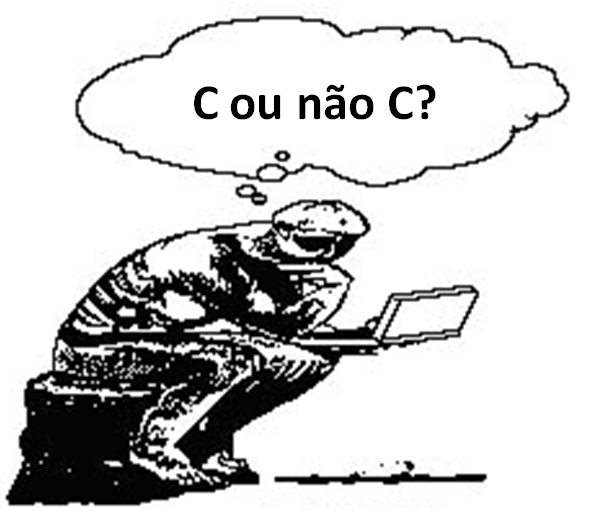
\includegraphics[width=7cm]{images/pensamento.png}
  		\end{center}
	\end{frame}
	
	\begin{frame}{Pensamento}
		\begin{columns}
			\column{.4\textwidth}  		
		  		\begin{center}
		    		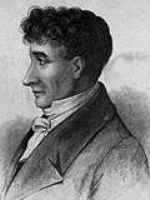
\includegraphics[width=.9\textwidth]{images/joubert.jpg}
		  		\end{center}
			\column{.6\textwidth}  		
				\begin{block}{Frase}
					\begin{center}
						{\large Jamais corte o que pode ser desatado.}
					\end{center}
				\end{block}		  		
		  		\begin{block}{Quem?}
		  			\begin{center}
						{\bf Joseph Joubert (1754 - 1824)} \\Moralista e ensaísta francês.
					\end{center}
				\end{block}
		\end{columns}
	\end{frame}
    
    \section{Revisão}
	
	\subsection{Grafos Bipartidos}
	\begin{frame}[shrink]{Grafo Bipartido}
		\begin{block}{Definição}
			Um grafo $G$ é {\bf bipartido} se existe uma bipartição $\{U, W \}$ de $V_G$ tal que toda aresta de $G$ tem uma ponta em $U$ e outra em $W$.
		\end{block}
		\begin{block}{Lembrando... Bipartição!}
			Uma bipartição de um conjunto $V$ é um par $\{U, W\}$ de conjuntos não vazios tal que $U \cup W = V$ e $U \cap W = \emptyset$.
		\end{block} 
		\begin{block}{Notação}
			\begin{itemize}
				\item Para explicitar a partição, podemos dizer que o grafo é {\bf $\{ U, W \}$-bipartido}.
				\item Se $G$ é um grafo $\{ U, W \}$-bipartido, podemos dizer, informalmente, que os elementos de $U$ são os {\bf vértices brancos} e os de $W$ são os {\bf vértices pretos} do grafo.
			\end{itemize}
		\end{block} 
	\end{frame}
	
	\begin{frame}{Grafo Bipartido}
		\begin{block}{Grafo $\{ U, W \}$-bipartido completo}
			Um grafo $\{U, W \}$-bipartido é {\bf completo} se todo vértice branco é adjacente a todos os vértices pretos. 
		\end{block}
		\begin{center}
			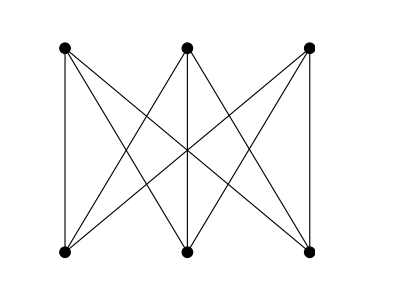
\includegraphics[width=.6\textwidth]{images/bipartido-completo.png}
		\end{center}
	\end{frame}
	
	\begin{frame}{Grafo Bipartido}
		\begin{block}{$K_{p,q}$}
			Um $K_{p,q}$ é um grafo bipartido completo com \\$p$ vértices brancos e $q$ pretos.
		\end{block} 
		\begin{block}{Estrela}
			\begin{itemize}
				\item Uma {\bf estrela} é um grafo $K_{1,q}$;
				\item Se $q \geq 2$, o {\bf centro} da estrela é o único vértice que incide em duas ou mais arestas;
				\item Se $q < 2$, a estrela não tem centro.
			\end{itemize}
		\end{block}
	\end{frame}
	
	\section{Caminhos e circuitos em grafos}
	\begin{frame}{Caminhos e circuitos em grafos}
		\begin{block}{Caminho em um grafo}
			Se um caminho $v_1 \ldots v_p$ é subgrafo de $G$, dizemos simplesmente que $v_1 \ldots v_p$ {\bf é um} caminho em $G$ ou que \\$G$ {\bf contém} o caminho $v_1 \ldots v_p$.
		\end{block} \pause
		\begin{exampleblock}{Circuitos em um grafo}
			Aplica-se identicamente a circuitos.
		\end{exampleblock} 
	\end{frame}
	
	\begin{frame}{Caminhos e circuitos em grafos}
		\begin{block}{Nomenclatura}
			Se $v$ e $w$ são os dois extremos de um caminho em $G$, é cômodo dizer que o caminho vai de $v$ a $w$ ou que começa em $v$ e termina em $w$.
		\end{block} \pause
		\begin{alertblock}{Cuidado!}
			Use estas expressões com cautela pois caminhos são objetos estáticos e não têm orientação.
		\end{alertblock}
	\end{frame}
	
	\begin{frame}{Caminhos e circuitos em grafos}
		\begin{block}{Caminho máximo em $G$}
			Um caminho $P$ em um grafo $G$ é máximo se $G$ não contém um caminho de comprimento maior que o de $P$.
		\end{block} \pause
		\begin{block}{Caminho maximal em $G$}
			Um caminho $P$ em $G$ é maximal se não existe caminho $P'$ em $G$ tal que $P \subset P'$.
		\end{block} \pause
		\begin{block}{Caminho Hamiltoniano}
			Um caminho é {\bf hamiltoniano} se contém todos os vértices do grafo.
		\end{block}
	\end{frame}	
	
	\section{Cortes}
	\begin{frame}{Cortes}
		\begin{block}{Definição}
			\begin{itemize}
				\item Suponha que $X$ é um conjunto de vértices de um grafo $G$. \pause
				\item O {\bf corte} associado a $X$ (ou {\bf franja} de $X$) é o conjunto de todas as arestas que têm uma ponta em $X$ e outra em $V_G \setminus X$.
			\end{itemize}
		\end{block} \pause
		\begin{block}{Notação}
			O corte associado a $X$ será denotado por
			\begin{center}
				$\partial_G (X)$
			\end{center}
		\end{block} \pause
		\begin{alertblock}{Outros autores...}
			Alguns preferem escrever $\delta(X)$ ou $\nabla(X)$.
		\end{alertblock}
	\end{frame}
	
	\begin{frame}{Cortes}
		\begin{block}{Cortes triviais}
			\begin{itemize}
				\item $\partial( \emptyset )$; \pause
				\item $\partial( V_G )$.
			\end{itemize}
		\end{block} \pause
		\begin{block}{Corolário}
			$|\partial(\{v\})| = d(v)$
		\end{block} \pause
		\begin{block}{Grau de um conjunto}
			\begin{itemize}
				\item Diremos que $|\partial(X)|$ é o {\bf grau} de $X$; \pause
				\item Denotamos este número como se segue:
					\begin{center}
						$d(X) := |\partial(X)|$
					\end{center}
			\end{itemize}
		\end{block}
	\end{frame}
	
	\begin{frame}{Cortes}
		\begin{block}{Corte - Definição}
			Um {\bf corte} ({\it = cut = coboundary}) em um grafo $G$ é qualquer conjunto da forma $\partial(X)$, em que $X$ é um subconjunto de $V_G$.
		\end{block} \pause
		\begin{alertblock}{Cuidado}
			Um corte é um conjunto de arestas, não de vértices.
		\end{alertblock}
	\end{frame}
	
	\begin{frame}
		\titlepage
	\end{frame}
	
\end{document}